\section{Медіана за каналами}

Щоб отримати цілісний знімок із мінімальною кількістю захмарених пікселів,
було використано медіану. Ця процедура на вхід отримує кілька знімків (рис. \ref{fig:composite-input})
та проходить по кожному каналу кожного знімка, формуючи єдине число, а
саме піксель окремого каналу. Причому ця медіана не змінює пікселі, які не
містять ніякої інформації (NODATA).

Таким чином створюється масив (4, x, y) (рис. \ref{fig:removal-result}), де x, y --- розмірність
вхідних знімків, а 4 --- це канали Red, Green, Blue та NIR.

\begin{figure}[H]
	\centering
	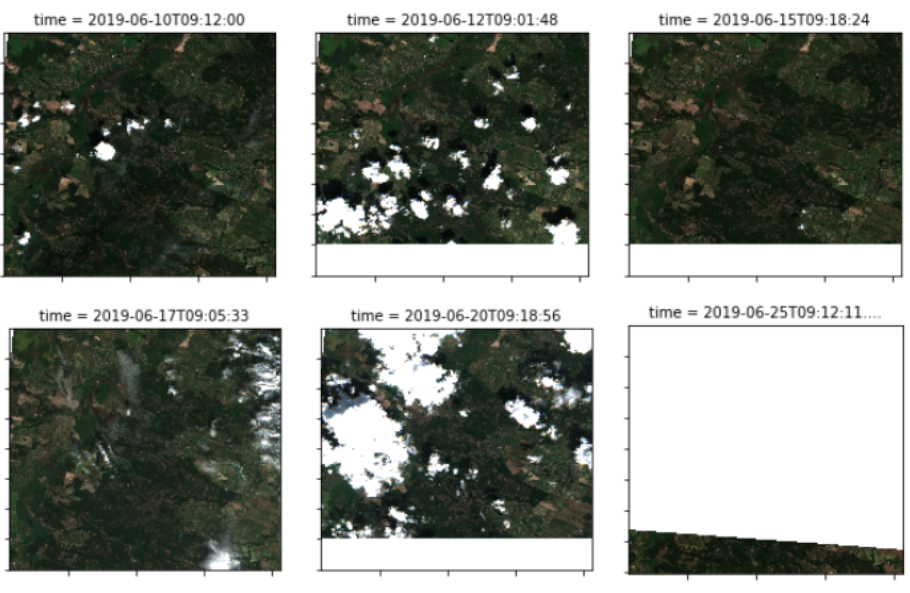
\includegraphics[width=0.7\textwidth]{images/image12}
	\caption{Вихідний набір даних для побудови композиту %
			(частина Київської області, знімки з '2019-05-31' по '2019-06-30')
	}
	\label{fig:composite-input}
\end{figure}

\begin{figure}[H]
	\centering
	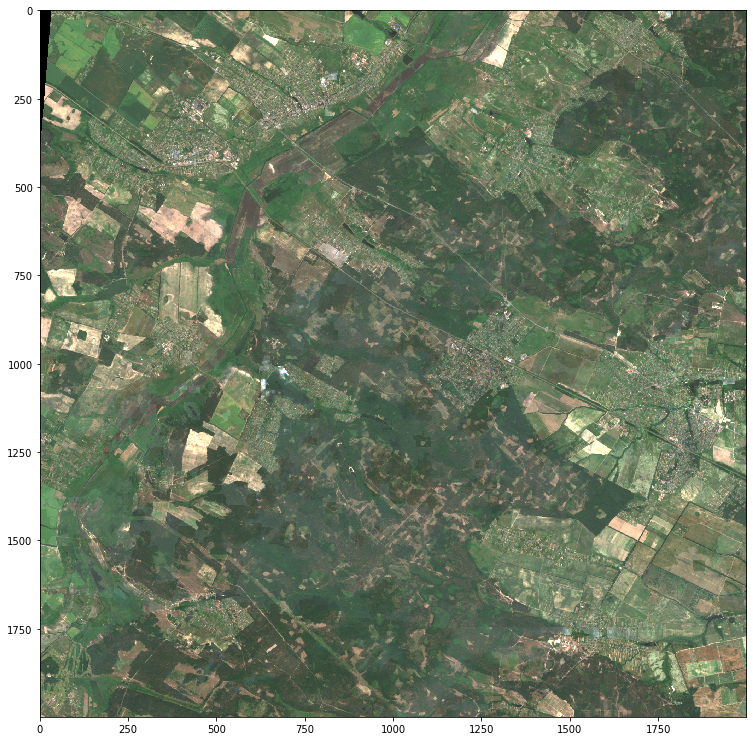
\includegraphics[width=0.6\textwidth]{images/image13}
	\caption{Графік залежності часу від кількості знімків для двох методів
	\label{fig:removal-result} }
\end{figure}
